% 
% exemplo genérico de uso da classe iiufrgs.cls
% $Id: iiufrgs.tex,v 1.1.1.1 2005/01/18 23:54:42 avila Exp $
% 
% This is an example file and is hereby explicitly put in the
% public domain.
% 
\documentclass[cic,tc]{iiufrgs}
% Para usar o modelo, deve-se informar o programa e o tipo de documento.
% Programas :
% * cic       -- Graduação em Ciência da Computação
% * ecp       -- Graduação em Ciência da Computação
% * ppgc      -- Programa de Pós Graduação em Computação
% * pgmigro   -- Programa de Pós Graduação em Microeletrônica
% 
% Tipos de Documento:
% * tc                -- Trabalhos de Conclusão (apenas cic e ecp)
% * diss ou mestrado  -- Dissertações de Mestrado (ppgc e pgmicro)
% * tese ou doutorado -- Teses de Doutorado (ppgc e pgmicro)
% * ti                -- Trabalho Individual (ppgc e pgmicro)
% 
% Outras Opções:
% * english    -- para textos em inglês
% * openright  -- Força início de capítulos em páginas ímpares (padrão da
% biblioteca)
% * oneside    -- Desliga frente-e-verso
% * nominatalocal -- Lê os dados da nominata do arquivo nominatalocal.def


% Use unicode
\usepackage[utf8]{inputenc}   % pacote para acentuação

% Necessário para incluir figuras
\usepackage{graphicx}         % pacote para importar figuras
\graphicspath{ {./figures/} }

\usepackage{times}            % pacote para usar fonte Adobe Times
% \usepackage{palatino}
% \usepackage{mathptmx}       % p/ usar fonte Adobe Times nas fórmula
\usepackage{listings}

\usepackage[alf,abnt-emphasize=bf]{abntex2cite}	% pacote para usar citações abnt

% 
% Informações gerais
% 
\title{Modelagem de ondas sísmicas através de paralelismo de tarefas}

\author{de Assis}{Lucas Barros}
% alguns documentos podem ter varios autores:

% orientador e co-orientador são opcionais (não diga isso pra eles :))
\advisor[Prof.~Dr.]{Schnorr}{Lucas Mello}

% a data deve ser a da defesa; se nao especificada, são gerados
% mes e ano correntes
% \date{maio}{2001}

% o local de realização do trabalho pode ser especificado (ex. para TCs)
% com o comando \location:
\location{Porto Alegre}{RS}

% 
% palavras-chave
% iniciar todas com letras minúsculas, exceto no caso de abreviaturas
% 
\keyword{programação paralela}
\keyword{programação baseada em tarefas}
\keyword{Ondes3D}
\keyword{StarPU}

%\settowidth{\seclen}{1.10~}

% 
% inicio do documento
% 
\begin{document}

% folha de rosto
% às vezes é necessário redefinir algum comando logo antes de produzir
% a folha de rosto:
% \renewcommand{\coordname}{Coordenadora do Curso}
\maketitle

% dedicatoria
% \clearpage
% \begin{flushright}
%     \mbox{}\vfill
%     {\sffamily\itshape
%       ``If I have seen farther than others,\\
%       it is because I stood on the shoulders of giants.''\\}
%     --- \textsc{Sir~Isaac Newton}
% \end{flushright}

% agradecimentos
%\chapter*{Agradecimentos}
%Agradeço ao \LaTeX\ por não ter vírus de macro\ldots



% resumo na língua do documento
\begin{abstract}
  A aplicação \textit{Ondes3D} tem como objetivo realizar a simulação da propagação de uma onda sísmica. Apesar de contar com uma implementação paralela
  utilizando \textit{OpenMP}, esse paralelismo só é obtido dentro de cada um de seus \textit{macro-kernels}.
  O trabalho aqui apresentado estuda as alterações necessárias para dividir as estruturas utilizadas pelo simulador em ladrilhos, possibilitando
  posteriormente uma implementação em forma de tarefas utilizando a biblioteca \textit{StarPU}.
  Essa divisão em tarefas permite um controle da granularidade dos processos paralelos através do tamanho dos ladrilhos utilizados, o que leva à uma
  otimização dos acessos em memória. Além disso, é possível que diferentes etapas do processo sejam executadas simultaneamente graças às especificações
  das dependências que o modelo de programação em tarefas inclui. Dessa forma, espera-se alcançar uma execução que aproveita arquiteturas \textit{multi-core}
  de forma mais vantajosa que a versão original.
\end{abstract}

% resumo na outra língua
% como parametros devem ser passados o titulo e as palavras-chave
% na outra língua, separadas por vírgulas
\begin{englishabstract}{Seismic waves modelling through task-based programming}{Parallel programming. Task-based programming. Ondes3D. StarPU}
  The \textit{Ondes3D} simulator aims to simulate the propagation of a seismic wave. Even though it has a parallel implementation using
  \textit{OpenMP}, this parallelism is only achieved inside each of its macro-kernels.
  The study presented in this document studies the modifications needed to split the structures used by \textit{Ondes3D} in tiles, which
  allows a task-based implementation using the \textit{StarPU} library.
  By splitting the code in tasks, it becomes is possible to control the granularity of the parallel processes through the tile sizes, which
  enables a memory access optimization. Other than that, different steps of the computation can be executed simultaneously thanks to the
  dependency specifications from the task-based model. With these modifications, it may be possible to achieve an execution which exploits
  multi-core architectures even better than the original version.
\end{englishabstract}

% lista de figuras
\listoffigures

% lista de tabelas
\listoftables

% lista de abreviaturas e siglas
% o parametro deve ser a abreviatura mais longa
\begin{listofabbrv}{SPMD}
\item[CPU] Central Process Unit
\item[DAG] Directed Acyclic Graph
\item[GPU] Graphics Processing Unit
\item[HPC] High-Performance Computing
\item[MPI] Message Passing Interface
\end{listofabbrv}

% idem para a lista de símbolos
% \begin{listofsymbols}{$\alpha\beta\pi\omega$}
%     \item[$\sum{\frac{a}{b}}$] Somatório do produtório
%     \item[$\alpha\beta\pi\omega$] Fator de inconstância do resultado
% \end{listofsymbols}

% sumario
\tableofcontents

% aqui comeca o texto propriamente dito

% introducao
\chapter{Introdução}
Uma ferramenta importante para a mitigação dos riscos decorrentes de terremotos é a simulação da propagação de ondas sísmicas \cite{Dupros2010HighperformanceFS}.
A aplicação \textit{Ondes3D} realiza essa simulação através do método de diferenças finitas, utilizando a biblioteca \textit{OpenMP} para
produzir paralelismo local e o protocolo \textit{MPI} em contextos distribuídos. No entanto, o paralelismo local somente existe dentro de cada
\textit{macro-kernel}, isto é, não existe execução paralela entre diferentes etapas do cálculo. Uma alternativa possível para acelerar a execução pode ser alcançada
utilizando um modelo que permita um paralelismo ainda maior que o atual. 

A biblioteca \textit{StarPU} é uma alternativa atual que implementa a programação baseada em tarefas para obter paralelismo. Dentro dese modelo, uma tarefa consiste
em uma função cuja especificação inclui, além de seus parâmetros, os seus modos de acesso: somente leitura, somente escrita ou leitura e escrita. Essas tarefas são
incluídas ao longo do código e, baseando-se na ordem de inserção e nos modos de acesso de cada uma delas, a biblioteca \textit{StarPU} constrói um grafo acíclico
direcionado representando as dependências entre essas tarefas. Durante a execução do programa, esse grafo é utilizado para escalonar as tarefas conforme a disponibilidade dos
recursos computacionais.
Apesar de contar com uma implementação paralela, o modelo de programação utilizado na versão original da aplicação não explora o paralelismo tanto quanto seria possível devido à sua
incapacidade de considerar as dependências entre os dados utilizados. Ao utilizar o paradigma de tarefas, torna-se possível considerar essas dependências para que diferentes etapas
do algoritmo possam ser executadas simultaneamente, alcançando assim um paralelismo superior ao atualmente implementado.

Este trabalho tem como objetivo estudar e implementar as alterações necessárias para que o algoritmo existente seja executado na forma de tarefas, assim como avaliar o paralelismo
obtido ao utilizar esse paradigma.

\section{Contribuições}


\chapter{Trabalhos relacionados}

A aplicação \textit{Ondes3D} já foi objeto de estudo em outros trabalhos, frequentemente visando um melhor desempenho, mas passando também pela busca de um consumo energético 
mais eficiente. Além disso, outras aplicações também tiveram seu tempo de execução diminuído empregando a programação baseada em tarefas. Alguns desses trabalhos serão discutidos abaixo.

Boito et al. \cite{boito} verificaram que mais de $72\%$ do tempo de execução do \textit{Ondes3D} é gasto realizando operações de leitura e escrita. Três otimizações diferentes foram
propostas: incialmente, uma camada de \textit{software} foi criada para centralizar as solicitações de entrada e saída da aplicação. Em um segundo momento, os passos de comunicação foram
substituídos por escritas diretas no sistema de arquivos. A terceira implementação passa a utilizar diversos arquivos de saída, o que permite que diversas operações de escrita aconteçam
paralelamente. Apesar dos resultados impressionantes desse trabalho, o estudo aqui proposto não tem como foco as operações de entrada e saída mas sim a paralelização dos cálculos
das equações elastodinâmicas, o que permitiria em um momento futuro a combinação das duas otimizações para alcançar uma aceleração ainda mais significativa.

Tesser et al. \cite{dupros:hal-00797682}, partindo de uma implementação distribuída em que o domínio é dividido em partes menores,  perceberam que o tempo de cálculo das equações
depende da região sendo tratada, causando um desbalanceamento de cargas entre os processadores utilizados. Ao utilizar uma implementação de \textit{MPI} construída sobre um suporte
de execução capaz de realizar um balanceamento dinâmico de tarefas, foi possível reduzir o tempo de execução em $23\%$. O presente estudo não considera a utilização de programação
distribuída, mas a granularidade parametrizável alcançada utilizando o modelo proposto permite uma mitigação dos efeitos de uma distribuição desbalanceada. Quanto maior o número de tarefas
disponível em um dado momento, menores são as chances de uma unidade de cálculo permanecer ociosa.

Castro et al. \cite{CASTRO2016108} utilizaram um processador de baixa potência para propor uma implementação da aplicação \textit{Ondes3D} com um baixo consumo energético. A partir
de uma estratégia de ladrilhamento multi-nível, a versão desenvolvida para o processador \textit{MPPA-256} apresentou uma diminuição de $86\%$ do consumo quando comparada à uma
execução em um processador convencional. No entanto, o consumo energético não é um fator considerado no estudo aqui apresentado.

Nesi et al. \cite{nesi} realizaram três implementações diferentes de uma aplicação de dinâmica de fluídos utilizando programação baseada em tarefas através da biblioteca \textit{StarPU}.
Além de incluir tarefas voltadas para \textit{GPU}s, o traço de execução resultante foi avaliado e refinado utilizando o conjunto de ferramentas \textit{StarVZ}. Utilizando a técnica de
células fantasma, explicada na seção \ref{sec:proposal}, foi possível alcançar uma aceleração de $77$x em relação à versão original.

Martínez et al. \cite{victor} propuseram uma implementação utilizando a biblioteca \textit{StarPU}, baseada em tarefas e considerando arquiteturas heterogêneas compostas por
\textit{CPU}s e \textit{GPU}s. De um certo modo essa proposta vai além da pesquisa aqui apresentada, onde não existe uma implementação voltada para \textit{GPU}. No entanto, Martínez et al.
optaram por descartas as interações com as bordas do domínio devido a complexidade introduzida pelo uso delas. A melhor performance foi alcançada utilizando quatro \textit{CPU}s e oito
\textit{GPU}s, uma aceleração de $25$x em relação à versão original utilizando doze \textit{CPU}s.


A Tabela \ref{tbl:related_works} resume as diferenças entre os trabalho desenvolvido e os estudos citados acima. Os projetos desenvolvidos por Nesi et al. e Martínez et al. são
os que mais se assemelham ao aqui desenvolvido, apesar do primeiro tratar de uma aplicação diferente e o segundo ignorar uma parcela da simulação.

\begin{table}[htb!]
    \caption{Trabalhos relacionados}
    \begin{center}
        \begin{tabular}{l|l|p{60mm}}
            \textit{Trabalho} & \textit{Aplicação} & \textit{Contexto} \\
            \hline
            \hline
            Boito et al.    & \textit{Ondes3D} & Otimização de operações de entrada e saída \\
            Tesser et al.   & \textit{Ondes3D} & Balanceamento dinâmico de carga             \\
            Martínez et al. & \textit{Ondes3D} & Implementação baseada em tarefas em arquiteturas heterogêneas sem condições de borda             \\
            Castro et al.   & \textit{Ondes3D} & Otimização de consumo energético             \\
            Nesi et al.     & Dinâmica de fluídos & Implementação baseada em tarefas em arquiteturas heterogêneas \\
            Este trabalho   & \textit{Ondes3D} & Implementação baseada em tarefas             \\
            \hline
        \end{tabular}
    \end{center}
    \legend{Fonte: Autor}
    \label{tbl:related_works}
\end{table}

\chapter{Fundamentação teórica}
Para a elaboração desse estudo, primeiramente é necessário compreender o que é a aplicação utilizada. A partir desse conhecimento, é possível tratar do modelo de programação
baseada em tarefas e como ela é implementada na biblioteca \textit{StarPU}. Finalmente, é necessário explicar o método de divisão das estruturas de dados usadas, conhecido como
ladrilhamento ou \textit{tiling}.

\section{Ondes3D}
A aplicação discretiza o mundo real em diversos tensores tri-dimensionais, endereçados a partir de suas coordenadas. Esses tensores são parte de diferentes estruturas de dados,
que podem variar de acordo com os dados experimentais utilizados na simulação.

Esse trabalho toma como objeto de estudo os dados do terremoto de \textit{Chuetsu-Oki},
que atingiu a costa japonesa em 2007. Nesse caso, a aplicação conta com as seguintes estruturas, usadas para representar os fenômenos físicos que compõem a onda:

\begin{itemize}
\item{\textit{STRESS}:} composta por tensores que representam as tensões sofridas em diferentes planos. O tensor \textit{xy}, por exemplo, representa a tensão sofrida no plano
  X - aquele cuja normal aponta na direção do eixo X, isto é, o plano YZ - pelas forças causadas na direção Y.
\item{\textit{VELOCITY}:} composta por tensores que representam a velocidade da onda nas direções X, Y e Z.
\item{\textit{SOURCE}:} composta pelos dados que descrevem a(s) fonte(s) da onda, como seu hipocentro, a longevidade da fonte, sua orientação e força.
\item{\textit{MEDIUM}:} composta pelos dados que descrevem o meio por onde a onda se propaga, como sua profundidade.
\item{\textit{ABSORBING BOUNDARY CONDITION}:} composta por vetores que representam as contribuições das bordas do domínio nos cálculos de tensão e velocidade. Essas bordas são
  utilizadas para limitar o domínio computacional onde o cálculo é feito gerando o mínimo de interferência nos cálculos realizados. \cite{ABCarticle}. 
\end{itemize}

Os cálculos são realizados seguindo um padrão \textit{stencil}, onde o valor atribuído aos tensores que descrevem as grandezas físicas são calculados usando informações
das células vizinhas. A Figura \ref{fig:stencil} ilustra um \textit{stencil} 2D com quatro vizinhos. Apesar da aplicação estudada usar coordenadas nos eixos X, Y e Z, o mesmo
conceito pode ser expandido para o espaço tridimensional.

\begin{figure}[!htb]
    \caption{Representação de um \textit{stencil} 2D com quatro vizinhos}
    \begin{center}
      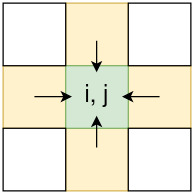
\includegraphics[width=6em]{stencil}
    \end{center}
    \label{fig:stencil}
    \legend{Fonte: Autor}
\end{figure}

As estruturas descritas anteriormente são atualizadas iterativamente, passando por quatro grandes etapas, também chamadas de \textit{macro-kernels}:

\begin{itemize}
\item{\textit{computeSeisMoment}:} etapa em que as fontes da onda são atualizadas
\item{\textit{computeIntermediates}:} etapa em que as contribuições das bordas do domínio são atualizadas a partir dos tensores de velocidade
\item{\textit{computeStress}:} etapa em que os tensores de tensão nos diferentes planos são atualizados a partir dos tensores de velocidade e das condições de borda
\item{\textit{computeVelocity}:} etapa em que os tensores de velocidade são atualizados a partir dos tensores de velocidade e das condições de borda
\end{itemize}

Com exceção da atualização das fontes da onda, que acontece em um domínio bastante restrito, os \textit{macro-kernels} descritos acima utilizam a diretiva \textit{omp parallel for}
para obter um paralelismo interno. Já que essas etapas realizam cálculos dentro de um laço triplo, iterando sob as coordenadas em X, Y e Z, a biblioteca \textit{OpenMP}, através
da diretiva citada anteriormente, cria \textit{threads} capazes de tratar diferentes coordenadas simultaneamente.

Teoricamente, a partir do momento que a tensão, por exemplo, de uma célula fosse calculada, já seria possível iniciar o cálculo de sua velocidade. No entanto, como a diretiva descrita acima 
não suporta o estabelecimento de dependências entre os dados, é necessário que a tensão de todas as células seja calculada para que o algoritmo possa iniciar a fase de cálculo
de velocidades. Dessa maneira, apesar da solução atual alcançar uma aceleração graças ao paralelismo introduzido, a quantidade de operações que podem ser executadas simultaneamente
é menor do que seria possível. O paralelismo baseado em tarefas busca explorar as dependências entre os dados para alcançar esse nível maior de independência entre as etapas do
algoritmo.

\section{Paralelismo baseado em tarefas}

O paralelismo baseado em tarefas é um modelo em que se busca descrever trechos de código paralelizáveis na forma de tarefas, que são criadas em tempo de execução pela biblioteca de
paralelismo utilizada. Depois de criar a tarefa, a biblioteca é responsável por executá-la ou adicioná-la a uma fila de tarefas para que ela seja executada em um momento apropriado.
A possibilidade de adiar a execução de uma tarefa é o que torna essa opção interessante ao considerarmos as dependências da aplicação aqui estudada.

\subsection{StarPU}

\textit{StarPU} é uma biblioteca de programação em tarefas para arquiteturas heterogêneas. Essa biblioteca foi criada visando atender à necessidade da comunidade de \textit{HPC} de
poder computacional \cite{StarPU}, criando uma ferramenta que facilita a criação de tarefas para diferentes arquiteturas e a especificação dos dados utilizados. No caso do estudo aqui
descrito, essa biblioteca é especialmente interessante ao determinar o momento de execução de suas tarefas, já que a escolha do momento de sua execução é baseada nas dependências de dados
existentes entre elas.

A utilização de tarefas é composta por dois momentos, sendo o primeiro deles a sua descrição e o segundo a sua inserção na fila de tarefas. O paralelismo obtido é o resultado da inserção de
diversas instâncias da mesma tarefa atuando sobre dados diferentes e tendo sua ordem de execução determinada pelas dependências entre elas.

A criação de uma tarefa começa pela construção de seu \textit{kernel}, uma função que implementa a tarefa a ser executada e que deve seguir a seguinte interface:

\begin{verbatim}
void task_name(void *buffers[], void *cl_arg)
\end{verbatim}

Nessa interface, os \textit{buffers} representam os dados que serão gerenciados pela biblioteca levando em conta suas dependências e modos de leitura. Já a estrutura
\textit{cl\_arg} guarda ponteiros de valores externos utilizados pelo \textit{kernel}, tipicamente valores constantes.

Com o \textit{kernel} criado, utiliza-se uma estrutura chamada \textit{codelet} para descrever a tarefa. Nessa estrutura é indicada a quantidade de \textit{buffers} utilizados
pela tarefa, seus modos de acesso e o nome dos \textit{kernels} que implementam-na. Voltando ao exemplo da função \textit{computeIntermediates}, um \textit{codelet}
possível é mostrado na Figura \ref{fig:intermediates_cl}.

\begin{figure}[!htb]
    \caption{Definição do \textit{codelet} da função \textit{computeIntermediates}}
    \begin{center}
      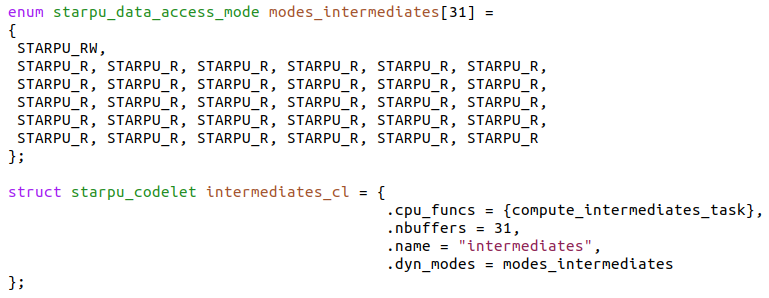
\includegraphics[width=25em]{intermediates_cl}
    \end{center}
    \label{fig:intermediates_cl}
    \legend{Fonte: Autor}
\end{figure}

A criação de instâncias de tarefas é feita através da função \textit{starpu\_insert\_task}, tendo como parâmetros o \textit{codelet} correspondente, os \textit{buffers} utilizados e
os ponteiros registrados como \textit{cl\_args}. 

A biblioteca segue o modelo de \textit{sequential task flow}, que permite que um fluxo paralelo seja facilmente descrito através de um algoritmo sequencial. As tarefas são submetidas
sequencialmente e, a partir de sua ordem de submissão e suas dependências, cria-se um grafo acíclico direcionado (também chamado de \textit{Directed Acyclic Graph}, ou \textit{DAG})
que descreve a hierarquia existente entre elas. A partir desse grafo, é possível escalonar as tarefas em tempo de execução de maneira que todas as dependências sejam respeitadas e o
tempo ocioso nas unidades de cálculo seja o menor possível.

\subsection{Matrizes \textit{ladrilhadas}}

Uma estratégia recorrente na programação de alta performance é o ladrilhamento de matrizes - no caso desse estudo, de tensores. Essa técnica consiste, conforme ilustra a Figura \ref{fig:tiled_matrix},
na divisão de uma matriz em sub-matrizes (também chamadas de blocos) de menor tamanho, indexadas pela sua posição em relação à matriz original.

\begin{figure}[!htb]
    \caption{Decomposição da matriz A em blocos}
    \begin{center}
      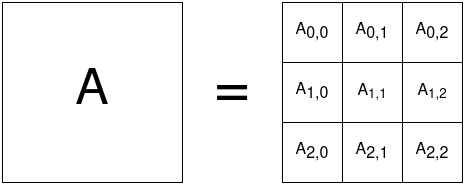
\includegraphics[width=15em]{tiled_matrix}
    \end{center}
    \label{fig:tiled_matrix}
    \legend{Fonte: Autor}
\end{figure}

O ladrilhamento de matrizes exige que os algoritmos sejam re-adequados à sua estrutura, mas em contrapartida oferecem numerosas vantagens. Em primeiro lugar, podemos citar a
otimização dos acessos em memória: ao utilizar um tamanho de bloco suficientemente pequeno, é possível que, durante a execução do cálculo sobre cada um dos blocos, todos os dados
necessários estejam presentes simultaneamente na memória cache. Além disso, utilizando o DAG criado por ferramentas como a biblioteca \textit{StarPU}, é possível executar
simultaneamente tarefas de etapas diferentes, acelerando ainda mais a execução da aplicação.

A Figura \ref{fig:gemm} ilustra o cálculo de multiplicação de matrizes utilizando matrizes ladrilhadas. A versão convencional do algoritmo consiste em acumular a soma dos produtos de
cada linha por cada coluna das matrizes envolvidas. Apesar dos elementos consecutivos de uma mesma linha encontrarem-se tipicamente lado a lado em memória, os saltos realizados nas trocas
de linha podem exigir uma reescrita completa da cache.

\begin{figure}[!htb]
    \caption{Algoritmo de multiplicação de matrizes por blocos}
    \begin{center}
      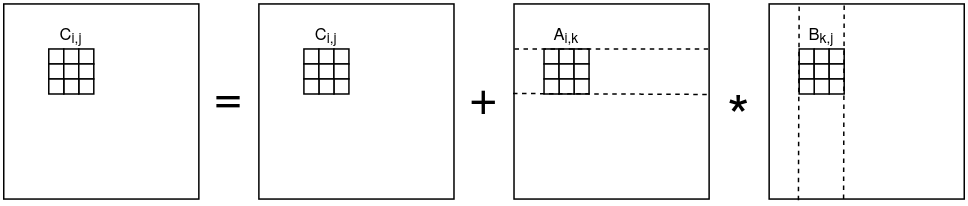
\includegraphics[width=25em]{gemm}
    \end{center}
    \label{fig:gemm}
    \legend{Fonte: Autor}
\end{figure}

A versão ladrilhada é composta por diversas execuções do algoritmo convencional, atuando sobre uma linha (respectivamente, coluna) de blocos de cada vez. Dessa forma, além de otimizar os
acessos de memória ao realizar pequenas multiplicações bloco a bloco, é possível executar simultaneamente o cálculo de todos os bloco da matriz resultante. Apesar dos blocos das matrizes
$A$ e $B$ serem acessados por diversas tarefas, eles não sofrem nenhuma escrita. Os blocos da matriz $C$, onde as escritas são realizadas, são acessados cada um deles por uma única tarefa,
possibilitando tal paralelismo.

\chapter{Projeto e implementação}
Neste capítulo serão apresentadas as alterações necessárias para que a aplicação \textit{Ondes3D} seja paralelizável na forma de tarefas gerenciadas pela biblioteca \textit{StarPU}.
Posteriormente, será apresentada uma descrição da implementação realizada ao longo dessa pesquisa.

\section{Proposta}\label{sec:proposal}

Os diversos tensores que representam as grandezas utilizadas nas equações elastodinâmicas do problema deverão ser divididos, de forma parametrizável, em blocos de tamanho igual.
A Figura \ref{fig:cuboids} ilustra o particionamento descrito utilizado pela implementação original, que parte de um arquivo de topologia para discretizar o plano $XY$ em blocos de profundidade
igual à do domínio.

\begin{figure}[!htb]
    \caption{Representação do espaço particionado em nove blocos}
    \begin{center}
      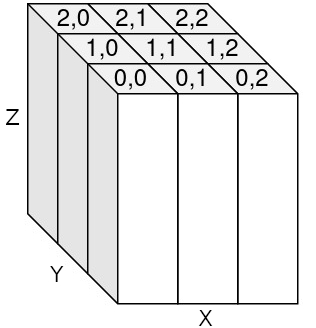
\includegraphics[width=10em]{cuboids}
    \end{center}
    \label{fig:cuboids}
    \legend{Fonte: Autor}
\end{figure}

Em relação ao laço principal de execução, a Figura \ref{fig:main_loop} resume o fluxo da aplicação original. O domínio do problema é dividido em cinco regiões denominadas \textit{imodes},
sendo quatro delas as linhas e colunas externas do domínio e a quinta os elementos internos. Com exceção da etapa \textit{computeSeisMoment}, cada \textit{macro-kernel} é executado cinco
vezes, uma em cada região. Internamente, cada etapa percorre o espaço [$x_{min}$, $x_{max}$][$y_{min}$, $y_{max}$][$z_{min}$, $z_{max}$].

\begin{figure}[!htb]
    \caption{Laço principal da aplicação original}
    \begin{center}
      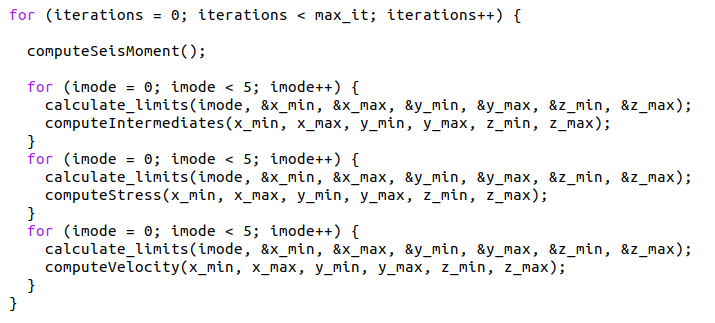
\includegraphics[width=28em]{main_loop}
    \end{center}
    \label{fig:main_loop}
    \legend{Fonte: Autor}
\end{figure}

Na versão aqui proposta, cada etapa será executada tantas vezes quanto houverem blocos. Para isso, será necessário iterar sobre os blocos disponíveis, criando uma tarefa para cada bloco
de dados, conforme mostra a Figura \ref{fig:new_main_loop}, dispensando a utilização dos \textit{imodes}. Neste momento vale ressaltar que a inserção das tarefas consiste
simplesmente na criação de uma instância de tarefa com as dependências indicadas e não implica em sua execução imediata. Fica a cargo da biblioteca \textit{StarPU} iniciar a execução
de cada uma das tarefas disponíveis de maneira assíncrona.

\begin{figure}[!htb]
    \caption{Laço principal da proposta}
    \begin{center}
      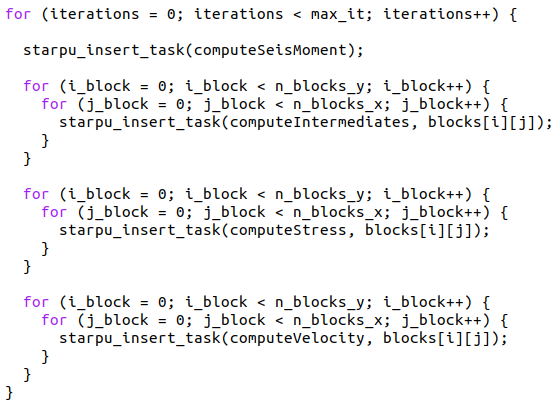
\includegraphics[width=25em]{new_main_loop}
    \end{center}
    \label{fig:new_main_loop}
    \legend{Fonte: Autor}
\end{figure}

Internamente, cada tarefa percorrerá apenas o espaço determinado pelo tamanho de bloco utilizado em vez de uma região completa como na versão original.

A utilização de blocos independentes introduz, no entanto, uma dificuldade nas aplicações do tipo \textit{stencil}: os elementos nas bordas de cada um dos blocos terão como vizinhos
elementos de outros blocos. Uma primeira solução, mais simples e menos eficiente, consiste em não utilizar somente um bloco por tarefa, mas sim cinco - o bloco a ser calculado, em
modo de leitura e escrita, e os seus quatro vizinhos imediatos, em modo leitura. Essa alternativa, dependendo do contexto em que ela é utilizada, pode representar um custo de memória mais
elevado do que o necessário. Uma solução mais eficiente é a utilização das chamadas \textit{ghost cells}. Já que é necessário ler apenas as células de uma borda de cada um dos vizinhos, em
vez de utilizar os quatro vizinhos completos, compartilha-se apenas as bordas que serão necessárias. A Figura \ref{fig:ghost_cells} mostra um exemplo de células fantasma em um \textit{stencil} 2D,
mas o conceito pode ser expandido para três dimensões.

\begin{figure}[!htb]
    \caption{Representação do uso de células fantasma}
    \begin{center}
      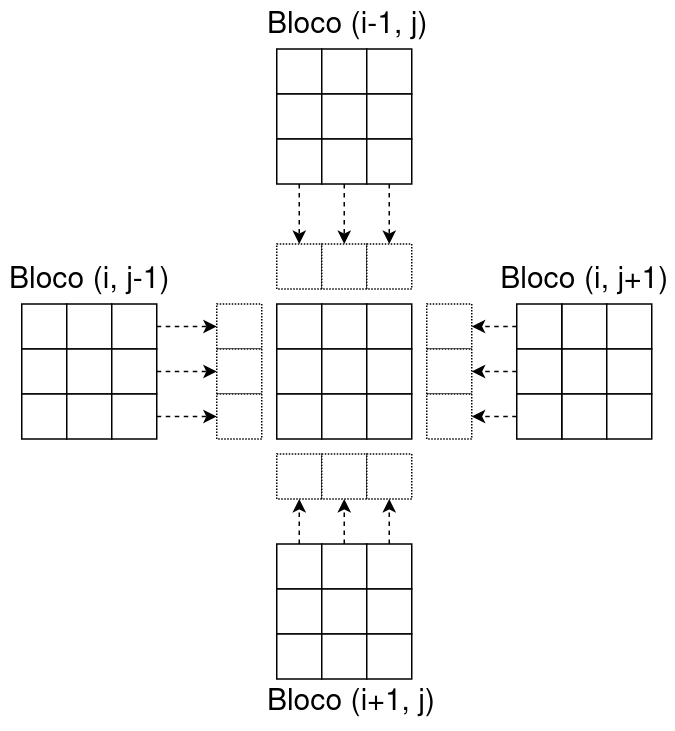
\includegraphics[width=16em]{ghost_cells}
    \end{center}
    \label{fig:ghost_cells}
    \legend{Fonte: Autor}
\end{figure}

\section{Implementação}

A fim de explorar as dificuldades da implementação em forma de tarefas e de analisar o nível de paralelismo alcançável usando esse paradigma, uma versão da aplicação \textit{Ondes3D} foi
desenvolvida utilizando a biblioteca \textit{StarPU}. As subseções seguintes detalham o processo de implementação realizado.

\subsection{Inicialização}

O primeiro passo para adaptar o algoritmo desenvolvido de maneira a melhor aproveitar as interfaces oferecidas pela biblioteca \textit{StarPU} foi a adequação de seus vetores multidimensionais. Apesar
do uso de ponteiros múltiplos facilitar o acesso às estruturas, a biblioteca conta com funções que realizam o ladrilhamento dos dados a partir do número de blocos desejado. Portanto, optou-se por
transformar todos os vetores multidimensionais em vetores de tamanho equivalente.

Ainda tratando de vetores, a aplicação original realizava um acesso a partir de suas coordenadas, mesmo que estas possuíssem valores negativos. A figura \ref{fig:negative_index} mostra a
técnica utilizada para alcançar esse efeito. Os ponteiros que endereçavam essas estruturas apontavam não para a primeira posição alocada, como normalmente é feito, mas para o n-ésimo elemento,
sendo $n$ a coordenada de valor mais negativo. Devido à complexidade em manter essa implementação utilizando vetores unidimensionais, optou-se por empregar um endereçamento convencional.

\begin{figure}[!htb]
    \caption{Representação de um vetor que permite índices negativos}
    \begin{center}
      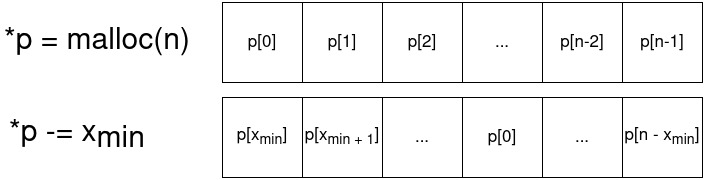
\includegraphics[width=28em]{negative_index}
    \end{center}
    \label{fig:negative_index}
    \legend{Fonte: Autor}
\end{figure}

Devido às mudanças de dimensionalidade e limites dos vetores, o acesso à essas variáveis se torna mais complexo. Para contornar esse problema, foram utilizadas macros que calculam o endereço
desejado a partir das dimensões do vetor acessado e das posições solicitadas.

** ipml, phiv e phit **

\subsection{Criação de \textit{buffers}}

*criaçao*
*filtros*
*unregister no final*

\subsection{Transformação em tarefas}
*leitura dos buffers com tamanho variavel (pontas)*
*coordenadas locais e globais*
*loop em ijk diferente*

\subsubsection{Acesso aos vizinhos}
*dados inteiros, blocos inteiros ou celulas fantasma*
*complexidade por ser stencil de grau 2*
*opçao de ler dados inteiros escrever em blocos*

\chapter{Avaliação experimental}
\section{Ambiente de testes}
\section{Resultados}

\chapter{Conclusão}

% e aqui vai a parte principal
% 
% \chapter{Estado da arte}
% \chapter{Mais estado da arte}
% \chapter{A minha contribuição}
% \chapter{Prova de que a minha contribuição é válida}
% \chapter{Conclusão}

% referências
% aqui será usado o environment padrao `thebibliography'; porém, sugere-se
% seriamente o uso de BibTeX e do estilo abnt.bst (veja na página do
% UTUG)
% 
% observe também o estilo meio estranho de alguns labels; isso é
% devido ao uso do pacote `natbib', que permite fazer citações de
% autores, ano, e diversas combinações desses

\bibliographystyle{abntex2-alf}
\bibliography{biblio}

\end{document}
